\chapter{Verwandte Arbeiten} \label{chap:relatedwork}

Das dritte Kapitel behandelt die Themen \emph{MegaDetector} und \emph{EfficientNet}. Während ersterer im Rahmen dieser Arbeit zur Lokalisierung von Tieren dient, kommt letzteres zur Klassifikation von Tieren zum Einsatz. 

\section{MegaDetector} \label{sec:megadetector}

\begin{figure}[!hb]
	\centering
	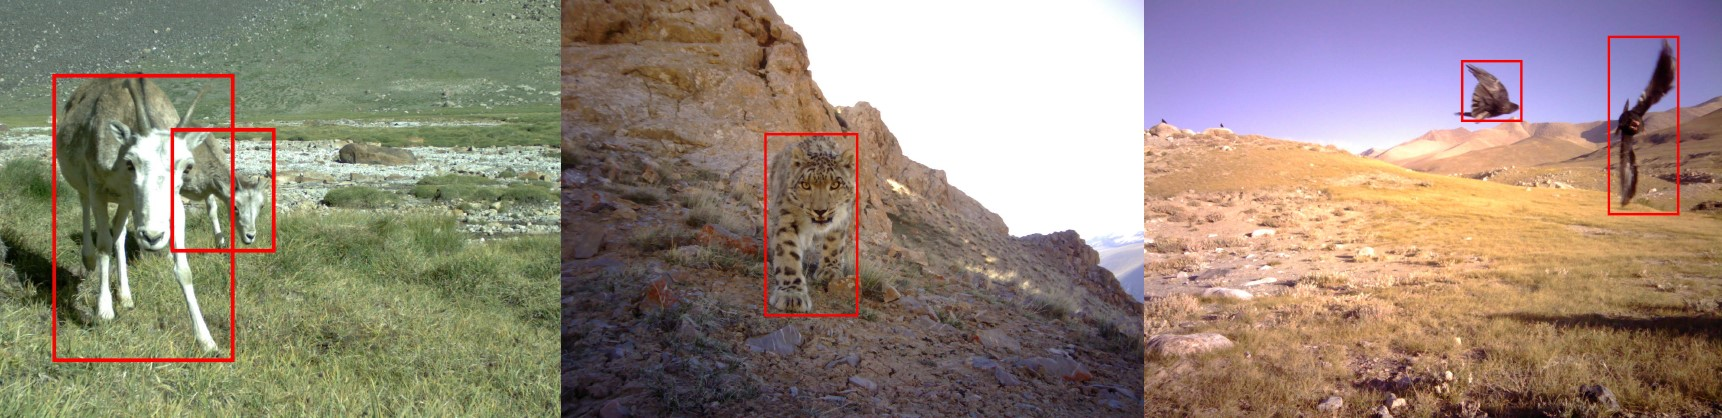
\includegraphics[width=\linewidth]{images/Megadetector example}
	\caption{Beispielergebnisse vom MegaDetector \protect\cite{beery2019efficient}}
	\label{fig:Megadetectorexample}
\end{figure}

Die Tierarterkennung lässt sich in die \emph{Tierlokalisierung} und die \emph{Tierklassifizierung} unterteilen. Für die Lokalisierung von Tieren wird in dieser Arbeit der MegaDetector \cite{beery2019efficient} angewendet, was ein CNN-Modell ist, das auf den Architekturen Faster-RCNN \cite{ren2016faster} und InceptionResNetv2 \cite{szegedy2016inceptionv4} basiert. Der MegaDetector wurde im Rahmen des Projekts \emph{AI for Earth}\footfullcite{AIforEarth} entwickelt und ist kein vortrainiertes, sondern ein vollständiges einsetzbares Modell. Grundsätzlich scannt der MegaDetector die Eingabebilder und gibt die Lokalisierungsergebnisse jedes Bildes (im Weiteren als \emph{MegaDetections} bezeichnet) in eine JSON-Datei aus. Eine MegaDetection enthält Informationen über die Position eines lokalisierten Tiers im Eingabebild sowie den entsprechenden Confidence-Wert der Lokalisierung. Im Folgenden wird beschrieben, welche Vorteile sich aus der Verwendung des MegaDetectors ergeben.

\begin{description}
	\item[Mögliche Lokalisierung von während des Trainings nicht gesehenen Tierarten]
	
	Theoretisch ist es möglich, ein bestehendes Modell neu zu trainieren, um fehlende Tierarten hinzuzufügen, aber in der Praxis ist dies schwierig und erfordert genauso viel Kosten wie das Trainieren eines Modells von Grund auf. Durch diesen Vorteil des MegaDetectors kann man Zeit sowie Ressourcen sparen.
	
	\item[Beschleunigung der Überprüfung von Kamerafallenbildern]
	
	%Im Testgebiet vom Projekt Natur 4.0 werden Kamerafallen installiert. Diese sind wärme- oder bewegungsaktivierte Kameras, die in freier Wildbahn platziert werden, um Tierpopulationen und ihr Verhalten zu überwachen und untersuchen. 
	
	Aufgrund einer hohen Rate an falschen Triggern sind auf den meisten Kamerafallenbildern keine Tiere sichtbar, was dazu führt, dass Experten viel Zeit in die Überprüfung von solchen Bildern investieren müssen.	Der MegaDetector löst dieses Problem, indem er die Kamerafallenbilder einliest und eine Liste von MegaDetections ausgibt. Bilder, die keine MegaDetections haben, gelten als leer und werden daher entfernt.
	
	\item[Generalisierbarkeit und Vereinfachung der anschließenden Klassifizierung]
	
	Der MegaDetector kann mit verschiedenen projektspezifischen Klassifizierern kombiniert werden, um verschiedene Projektziele zu verfolgen. Darüber hinaus vereinfacht der MegaDetector die anschließende Klassifizierung der lokalisierten Tiere. Da eine MegaDetection die Koordinaten eines Tiers umfasst, kann basierend darauf der Bildausschnitt mit dem Tier ausgeschnitten und den Klassifizierern übergeben werden (siehe \autoref{fig:MegadetectorRedFox}). Somit werden die verrauschten irrelevanten Pixel entfernt und folglich müssen sich die Klassifizierer nur um Tierpixel kümmern.
	
	\begin{figure}[!h]
		\centering
		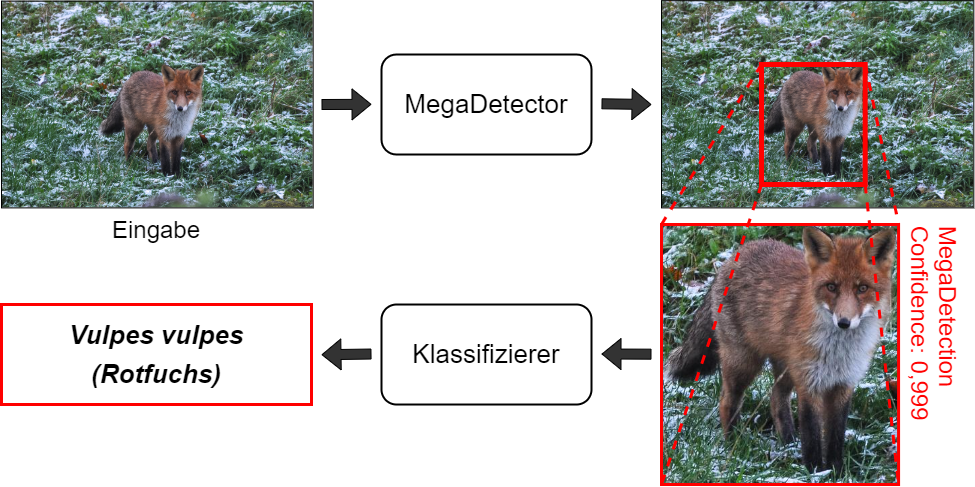
\includegraphics[width=\linewidth]{images/MegadetectorRedFox}
		\caption{Visuelle Erkennung eines Rotfuchses. Die Klassifizierung ist dank der Entfernung des unnötigen Randbereichs einfacher.}
		\label{fig:MegadetectorRedFox}
	\end{figure}
	
\end{description}

Weitere Alternativen zur Tierlokalisierung anstelle des MegaDetector lassen sich in diesem Link\footfullcite{CameraTrapSurvey} finden. Jedoch haben diese Modelle einen oder mehrere der folgenden Nachteile:

\begin{itemize}
	\item Geschlossener Quellcode.
	
	\item Lokalisierung nur bestimmter Tierarten und nur in bestimmten Regionen.
	
	\item Unverfügbare oder nur manuelle Batchverarbeitung der Eingabebilder. Dies führt dazu, dass der Aufbau eines automatischen Modells zur visuellen Tierarterkennung unmöglich ist.
	
	\item Das Eingabeformat ist ausschließlich Video.
	
	\item Die Endergebnisse sind lediglich Bilder mit Bounding Boxes um die Tiere und es werden keine zusätzlichen hilfreichen Informationen zur Verfügung gestellt (z.~B. Koordinaten der Rahmen oder Confidence-Werte der Lokalisierung).
\end{itemize}

\section{EfficientNet} \label{sec:efficientnet}

Für die Klassifizierung der Tiere werden Modelle der CNN-Architektur EfficientNet benutzt. In diesem Abschnitt geht es um den Ausgangspunkt und Skalierungsansatz von EfficientNet sowie den Performanzvergleich zwischen EfficientNet- und anderen Modellen.

\subsection{Skalierung von CNNs}

Die Autoren von EfficientNet, Tan und Le, untersuchten in ihrem Artikel zu EfficientNet die zentrale Fragestellung: Gibt es eine \textit{prinzipielle} Methode, um CNNs zu skalieren, damit eine höhere Genauigkeit und Effizienz erreicht werden kann? Tan und Le beobachteten, dass obwohl die Leistung eines CNN-Modells durch einfaches Hochskalieren einer der drei Dimensionen Tiefe, Breite und Auflösung verbessert werden kann, ist dies jedoch nicht immer möglich:

\begin{description}
	\item[Tiefenskalierung] Die Tiefe eines CNN-Modells bezieht sich auf die Anzahl der Schichten darin. Je mehr Schichten (insbesondere Convolutional Layers) ein CNN-Modell hat, desto reichhaltigere und komplexere Merkmale kann das Modell aus dem Eingabebild extrahieren und lernen. Beispielsweise basieren beide CNN-Modelle ResNet-101 und ResNet-200 in \cite{cui2021parametric} auf der ResNet-Architektur von \cite{he2015deep}, aber da ResNet-200 viel tiefer ist als ResNet-101 (200 im Vergleich zu 101 Schichten), konnte ResNet-200 eine höhere Top-1 Accuracy als ResNet-101 erreichen (81,8\% im Vergleich zu 80,9\%)\footfullcite{ResNet200_101_PaperWithCodes}.
	
	Allerdings sind tiefere CNNs aufgrund vom \emph{Vanishing Gradient Problem}\footfullcite{VanishingGradientProblem} auch schwieriger zu trainieren \cite{zagoruyko2017wide}. Darüber hinaus verringert sich der Genauigkeitsgewinn ab einer gewissen Tiefe. Dies wurde durch die Autoren von EfficientNet in einer ihrer empirischen Untersuchungen in \autoref{fig:DiminishingScalingAccuracy} (Mitte) gezeigt.
	
	\item[Breitenskalierung] Diese Methode wird häufig benutzt, um CNN-Modelle untief zu halten. Die Breite eines CNN-Modells bezieht sich auf die Anzahl der Filter bzw. Feature-Maps pro Schicht (Die Regel lautet, dass sich aus jedem Filter eine Feature-Map ergibt). Allgemein führt eine Erhöhung der Anzahl von Filter (insbesondere denjenigen in Convolutional Layers) zu einer Erhöhung der Anzahl von Merkmalen, die extrahiert und gelernt werden können, und dadurch zu detaillierteren Merkmalen in höheren Schichten. Daneben sind breitere CNN-Modelle einfacher zu trainieren \cite{zagoruyko2017wide}. Typische breite CNN-Modelle sind \emph{WideResNet(-50-2-bottleneck)} in \cite{zagoruyko2017wide} sowie \emph{MobileNet(-224)} in \cite{howard2017mobilenets}, jeweils mit 78,1\% und 70.6\% ImageNet Top-1 Accuracy \cite{PapersWithCode-ImageNet}.
	
	Extrem breite und untiefe CNN-Modelle haben jedoch Schwierigkeiten beim Erfassen von Higher-Level-Merkmalen in höheren Schichten. Dabei verringert sich der Genauigkeitsgewinn ab einer gewissen Breite. Dies lässt sich durch die empirischen Untersuchungsergebnisse in \autoref{fig:DiminishingScalingAccuracy} (links) zeigen.
	
	\item[Auflösungsskalierung] Ein Bild mit höherer Auflösung enthält mehr Informationen als ein Bild mit niedrigerer Auflösung. Daher kann man die Architektur eines CNN-Modells ändern, damit das Modell ein größeres Eingabebild aufnehmen und dadurch eine bessere Leistung erzielen kann.
	Als Argument dafür haben Tan und Le das CNN-Modell \emph{GPIPE} aus \cite{huang2019gpipe} angeführt, das mit 480$\times$480 Auflösung im Gegensatz zu normalen 224$\times$224 84,4\% ImageNet Top-1 Accuracy erreichen konnte \cite{PapersWithCode-ImageNet}.
	
	Wie in den beiden vorherigen Fällen verringert sich der Genauigkeitsgewinn ab einer bestimmten Auflösung. \autoref{fig:DiminishingScalingAccuracy} (rechts) zeigt die Ergebnisse der Auflösungsskalierung eines CNN, wobei höhere Auflösungen die Genauigkeit verbessern, aber die Genauigkeitsverbesserung bei besonders hohen Auflösungen abnimmt ($r$=1,0 bezeichnet die Auflösung 224$\times$224 und $r$=2,5 bezeichnet die Auflösung 560$\times$560).
\end{description}

\begin{figure}[!h]
	\centering
	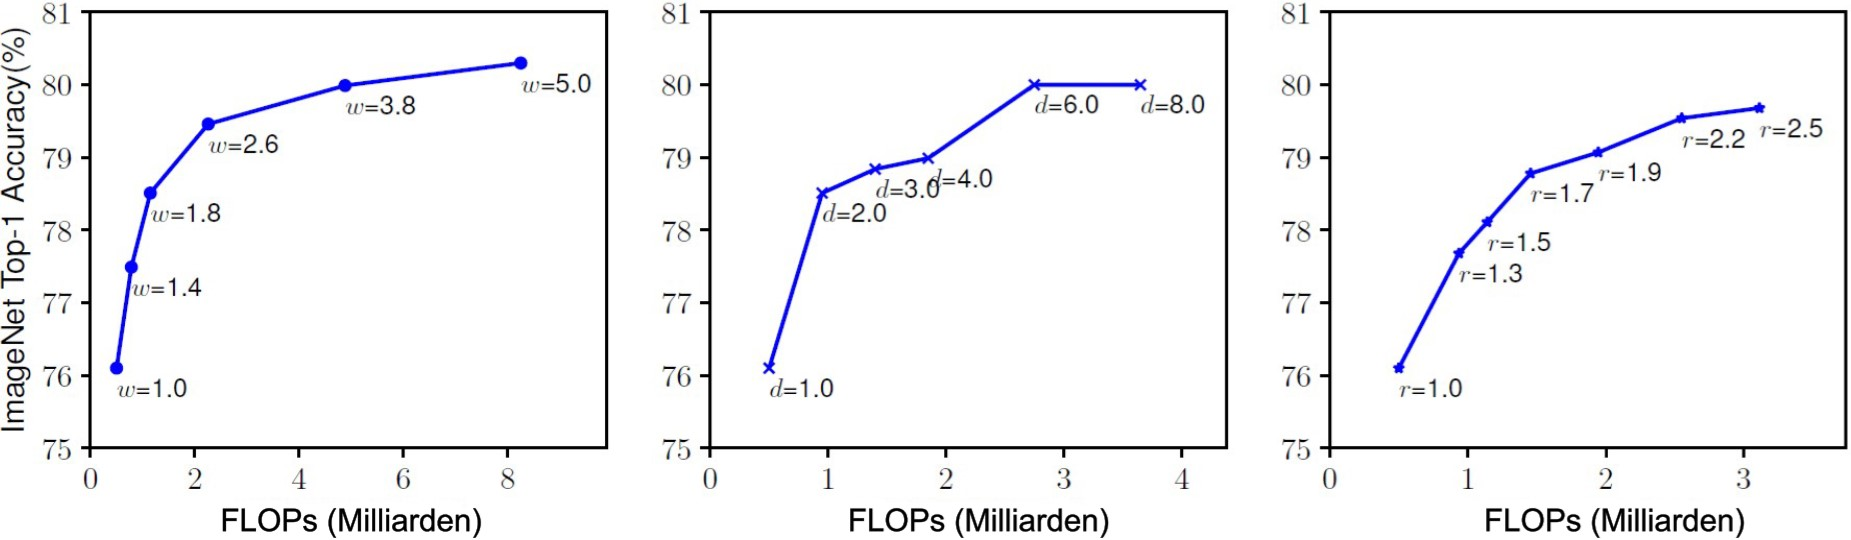
\includegraphics[width=\linewidth]{images/DiminishingScalingAccuracy}
	\caption{Hochskalieren eines CNN-Basismodells mit unterschiedlichen Breiten- ($w$), Tiefen- ($d$) und Auflösungskoeffizienten ($r$). Dabei bezeichnet die horizontale Achse die erforderlichen Kosten für das Training \emph{FLOPs}, d.~h. die benötigte Anzahl von Gleitkommaoperationen (\textbf{Fl}oating point \textbf{op}eration\textbf{s}). Größere Modelle mit größerer Breite, Tiefe oder Auflösung erzielen tendenziell eine höhere Genauigkeit, aber der Genauigkeitsgewinn wird nach Erreichen von 80\% schnell gesättigt, was die Einschränkung der eindimensionalen Skalierung zeigt. \protect\cite{tan2020efficientnet}}
	\label{fig:DiminishingScalingAccuracy}
\end{figure}

Außerdem haben die Autoren von EfficientNet beobachtet, dass es, um eine bessere Genauigkeit und Effizienz zu erzielen, wesentlich ist, während der CNN-Skalierung \textit{alle} Dimensionen Breite, Tiefe und Auflösung auszugleichen. Dies war eine Schlussfolgerung, die Tan und Le aus einer empirischen Untersuchung gezogen haben, deren Ergebnisse in \autoref{fig:ScalingWidthForDiffBaselineModels} dargestellt sind. Dabei haben die Autoren die Breitenskalierung unter verschiedenen Tiefen und Auflösungen verglichen. Wenn nur die Netzwerkbreite $w$ skaliert wurde, ohne die Tiefe und Auflösung zu ändern (d.~h. $d$=1,0 und $r$=1,0), sättigte die Genauigkeit schnell. Mit größerer Tiefe ($d$=2,0) und höherer Auflösung ($r$=1,3) erreichte die Breitenskalierung eine viel bessere Genauigkeit bei gleichen FLOPs-Kosten.

\begin{figure}[!h]
	\centering
	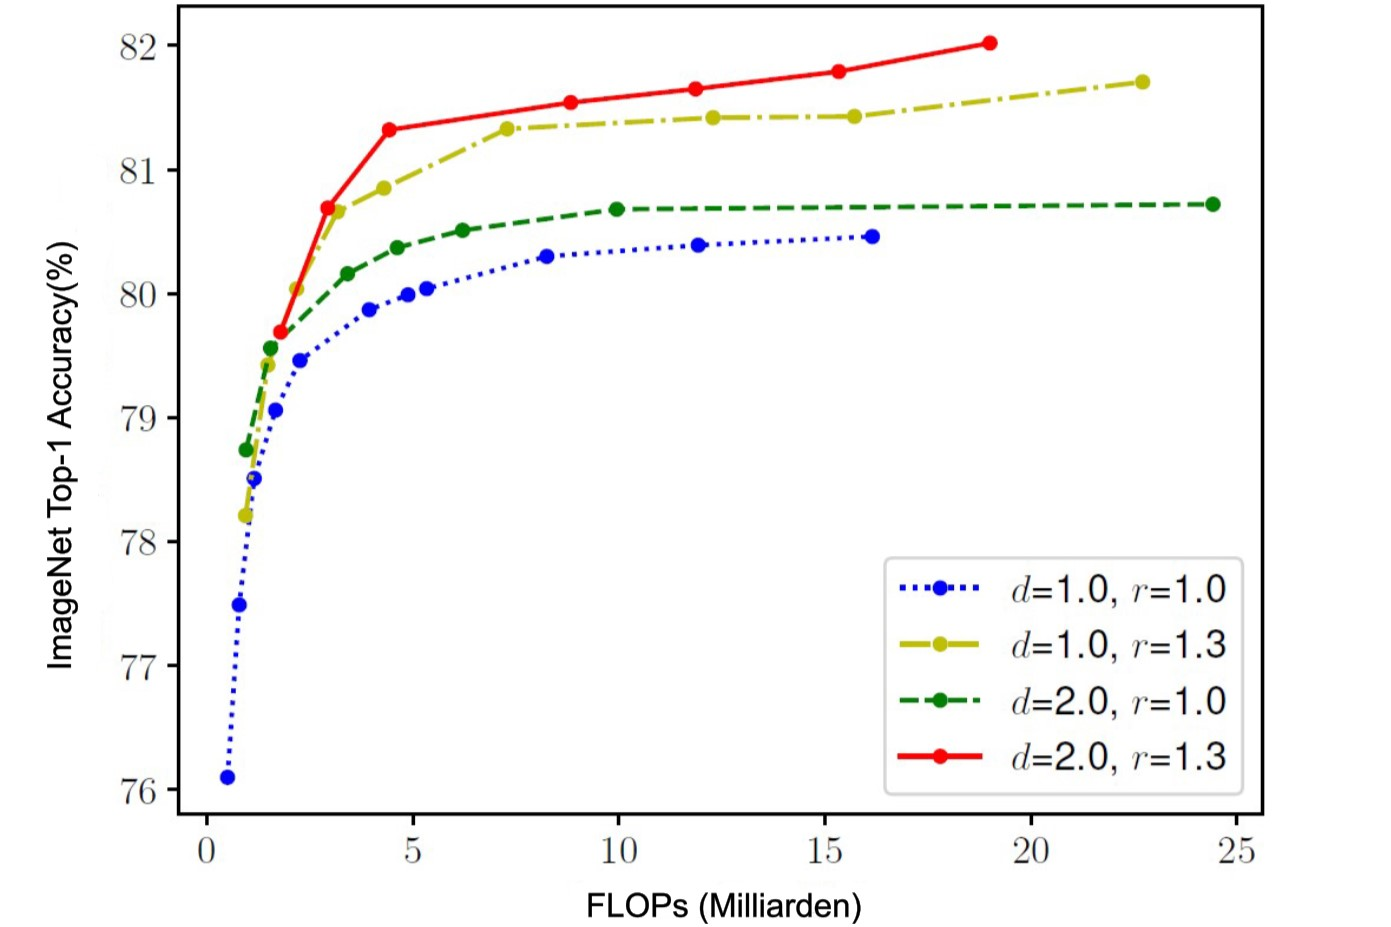
\includegraphics[width=\linewidth]{images/ScalingWidthForDiffBaselineModels}
	\caption{Breitenskalierung für verschiedene Basismodelle. Jeder Punkt in einer Linie bezeichnet ein Modell mit einem anderen Breitenkoeffizienten ($w$). \protect\cite{tan2020efficientnet}}
	\label{fig:ScalingWidthForDiffBaselineModels}
\end{figure}

Basierend auf den oberen Beobachtungen haben die Autoren von EfficientNet einen neuen Skalierungsansatz namens \emph{Compound Scaling} vorgeschlagen.

\subsection{Compound Scaling}

\begin{figure}[H]
	\centering
	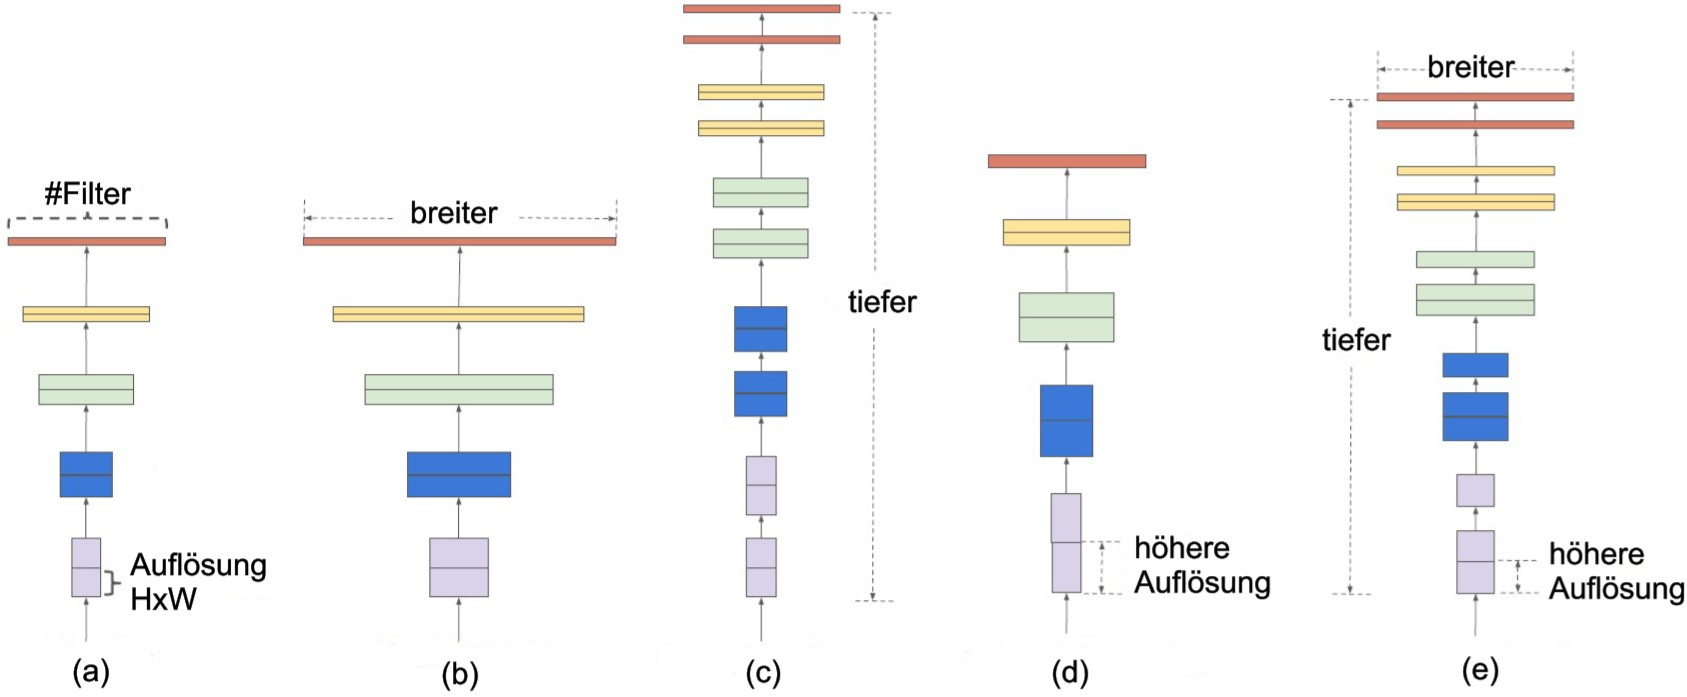
\includegraphics[width=\linewidth]{images/compoundScaling}
	\caption{Modellskalierung. (a) Basismodell; (b) Breitenskalierung; (c) Tiefenskalierung; (d) Auflösungsskalierung; (e) Compound-Scaling-Methode. \protect\cite{tan2020efficientnet}}
	\label{fig:compoundScaling}
\end{figure}

Die Compound-Scaling-Methode verwendet einen \emph{Compound-Koeffizienten} $\phi$, um Breite, Tiefe und Auflösung auf prinzipielle Weise gleichmäßig zu skalieren:

\begin{equation} \label{eq:compoundscaling}
	\begin{split}
		Tiefe: &\; d = \alpha^\phi \\
		Breite: &\; w = \beta^\phi \\
		Aufloesung: &\; r = \gamma^\phi \\
		mit &\; \alpha\cdot\beta^2\cdot\gamma^2 \approx 2 \\
		&\; \alpha \geq 1, \beta \geq 1, \gamma \geq 1
	\end{split}
\end{equation}

wobei $\phi$ ein benutzerdefinierter Koeffizient ist, der steuert, wie viel zusätzliche Ressourcen (z.~B. Gleitkommaoperationen – FLOPs) für die Modellskalierung verfügbar sind, während die konstanten Hyperparameter $\alpha, \beta, \gamma$ angeben, wie diese zusätzlichen Ressourcen der Breite, Tiefe bzw. Auflösung des Modells zugewiesen werden. 

In der Regel sind die erforderlichen Rechenkosten für das Training (d.~h. die benötigte Anzahl von FLOPs) direkt proportional zu den Koeffizienten $d, w^2, r^2$ und somit $(\alpha\cdot\beta^2\cdot\gamma^2)^\phi$. Dieser Schluss kommt von den Beobachtungen, dass die Verdopplung von Netzwerktiefe zur Verzweifachung der Rechenkosten führt, während die Verdopplung von Netzwerkbreite bzw. -auflösung die Vervierfachung der Rechenkosten zur Folge haben. In ihrer Arbeit haben die Autoren von EfficientNet  $\alpha\cdot\beta^2\cdot\gamma^2 \approx 2$ beschränkt, sodass sich für jeden neuen $\phi$ die benötigte Anzahl von FLOPs um das $2^\phi$-fache erhöht.

Die Compound-Scaling-Methode wurde nicht nur anhand bestehender CNNs evaluiert, sondern auch mittels eines Basismodells namens \emph{EfficientNet(-B0)}\footnote{Die genaueren Details zu der Architektur von EfficientNet-B0 befinden sich im originalen EfficientNet-Artikel \cite{tan2020efficientnet} und werden nicht in dieser Arbeit behandelt.} bewertet, das Tan und Le basierend auf der Architektur von \emph{MnasNet} in \cite{tan2019mnasnet} entwickelt haben. Das Modell ließ sich wie folgt hochskalieren:

\begin{enumerate}
	\item Der erste Schritt ist die Hyperparameteroptimierung, d.~h. die Suche nach den optimalen Hyperparametern $\alpha, \beta, \gamma$ für EfficientNet-B0. Dazu haben die Autoren eine \emph{Rastersuche}\footfullcite{liashchynskyi2019grid} mit $\phi$=1 durchgeführt. Sie fanden heraus, dass die besten Werte für EfficientNet-B0 $\alpha$=1,2, $\beta$=1,1 und $\gamma$=1,15 waren (unter der Bedingung $\alpha\cdot\beta^2\cdot\gamma^2 \approx 2$).
	
	\item Diese Werte von $\alpha, \beta, \gamma$ wurden anschließend als konstant gesetzt und ausgehend davon wurde das Hochskalieren vom Basismodell EfficientNet-B0 mit unterschiedlichen $\phi$-Werten durchgeführt. Daraus ergab sich eine Familie von Modellen namens \emph{EfficientNet-B1} bis \emph{-B7}, deren Leistungen im Vergleich zu anderen CNNs im nächsten Unterabschnitt detaillierter untersucht werden.
\end{enumerate}

\subsection{Leistungsvergleich}

Die \autoref{table:effnetaccu} zeigt, wie sich die EfficientNet-Modelle gegen andere Modelle bewähren. Zum Effizienzvergleich werden Modelle mit ähnlicher Top-1 Accuracy gruppiert. 

\begin{table}[!ht]
	\centering
	\caption{Vergleich zwischen Leistung sowie Kosten von EfficientNet- und anderen Modellen auf dem ImageNet-Validierungsdatensatz. Alle nicht kursiven Angaben werden von \cite{KerasRef} referenziert, während der Rest je nachdem aus entsprechenden Originalartikeln entnommen wird.}
	\label{table:effnetaccu}
	\begin{tabular}{l|c|>{\centering}m{1.7cm}c}
		
		\hline
		Modell & Top-1 Acc. (\%) & \#Params (Mio.) & Verhältnis-zu-EfficientNet \\
		
		\hline
		\textbf{EfficientNet-B0} & \textbf{77,19} & \textbf{5,3} & \textbf{1,0$\times$} \\
		%VGG16 \cite{simonyan2015deep} & 71,27 & 138,4 & 26,1$\times$ \\
		%NASNetMobile \cite{zoph2018learning} & 74,37 & 7,7 & 1,5$\times$ \\
		%MobileNetV2(alpha=1,4) \cite{sandler2019mobilenetv2} & 75,23 & 6,2 & 1,2$\times$ \\
		MobileNetV3(large) \cite{howard2019searching} & 75,56 & 5,5 & 1,0$\times$ \\
		%ResNet50V2 \cite{he2016identity} & 75,96 & 25,6 & 4,8$\times$ \\
		DenseNet169 \cite{huang2018densely} & 76,18 & 14,3 & 2,7$\times$ \\
		ResNet152 \cite{he2015deep} & 76,60 & 60,4 & 11,4$\times$ \\
		
		
		\hline
		\textbf{EfficientNet-B1} & \textbf{79,13} & \textbf{7,9} & \textbf{1,0$\times$} \\
		%DenseNet201 \cite{huang2018densely} & 77,32 & 20,2 & 2,6$\times$ \\
		InceptionV3 \cite{szegedy2015rethinking} & 77,90 & 23,9 & 3,0$\times$ \\
		ResNet152V2 \cite{he2016identity} & 78,03 & 60,4 & 7,6$\times$ \\
		ResNeXt101 \cite{xie2017aggregated} & 78,73 & 44,3 & 5,6$\times$ \\
		Xception \cite{chollet2017xception} & 79,01 & 22,9 & 2,9$\times$ \\
		
		
		\hline
		\textbf{EfficientNet-B2} & \textbf{80,18} & \textbf{9,2} & \textbf{1,0$\times$} \\
		\textit{WideNet-H} \cite{xue2021wider} & \textit{80,09} & \textit{63,0} & \textit{6,8$\times$} \\	
		
		
		\hline
		\textbf{EfficientNet-B3} & \textbf{81,58} & \textbf{12,3 } & \textbf{1,0$\times$} \\
		InceptionResNetV2 \cite{szegedy2016inceptionv4} & 80,26 & 55,9 & 4,5$\times$\\
		
		
		\hline
		\textbf{EfficientNet-B4} & \textbf{82,96} & \textbf{19,5} & \textbf{1,0$\times$} \\
		NASNetLarge \cite{zoph2018learning} & 82,50 & 93,5 & 4,8$\times$ \\
		
		
		\hline
		\textbf{EfficientNet-B5} & \textbf{83,70} & \textbf{30,6} & \textbf{1,0$\times$} \\	
		\textit{AmoebaNet-C} \cite{cubuk2019autoaugment} & \textit{83,50} & \textit{155,0} & \textit{5,1$\times$} \\		
		
		
		\hline
		\textbf{EfficientNet-B6} & \textbf{84,08} & \textbf{43,3 } & \textbf{1,0$\times$} \\
		\textit{AmoebaNet-A} \cite{real2019regularized} & \textit{83,90} & \textit{469,0} & \textit{10,8$\times$} \\			
		
		
		\hline
		\textbf{EfficientNet-B7} & \textbf{84,43} & \textbf{66,7} & \textbf{1,0$\times$} \\
		\textit{GPipe} \cite{huang2019gpipe} & \textit{84,40} & \textit{557,0} & \textit{8,4$\times$} \\
		\textit{ViT-L/16} \cite{dosovitskiy2021image} & \textit{87,76} & \textit{307,0} & \textit{4,6$\times$} \\	
		\hline
	\end{tabular}
\end{table}

Aus der Tabelle geht hervor, dass EfficientNet-Modelle alle anderen Modelle darin (mit Ausnahme vom letzten Eintrag) übertreffen. Die EfficientNet-B0 bis -B7 können nicht nur eine höhere Leistung erreichen, sondern auch die Anzahl der Parameter um eine Größenordnung (bis zu mehr als das Zehnfache) reduzieren. Dadurch lassen sich die Rechenlast, die Speichernutzung sowie die Gefahr von \emph{Overfitting}\footnote{Der Begriff verweist auf einen Effekt, der auftritt, wenn ein zu komplexes Modell neue Daten nicht gut vorhersagt, weil es an die Trainingsdaten übermäßig angepasst ist \cite{Novustat}.} senken. Diese Vorteile sprechen für den Einsatz von EfficientNet zur visuellen Erkennung von Tierarten im Projekt Natur 4.0.

Allerdings findet sich in \autoref{table:effnetaccu} ein Modell, das trotz höherer Parameteranzahl EfficientNet-B7 weit übertrifft (insbesondere um 3\% Top-1 Accuracy höher), nämlich \emph{ViT-L/16}. In der Tat gehört ViT-L/16 zu der im \autoref{chap:intro} erwähnten Architektur Vision-Transformer, die gemäß \cite{PapersWithCode-ImageNet} besser ist als EfficientNet hinsichtlich der besten Top-1 Accuracy, die jede Architektur erzielen kann. Es stellt sich daher die Frage, warum Vision-Transformer nicht in Natur 4.0 eingesetzt wird. Dafür gibt es zwei Gründe:

\begin{enumerate}
	\item Die Parameteranzahl von Vision-Transformer-Modellen ist gemäß \cite{PapersWithCode-ImageNet} extrem groß. Von den Top-20-Modellen in Bezug auf die Top-1 Accuracy sind sieben mit Vision-Transformer- und vier mit EfficientNet-Architektur. Die durchschnittliche Parameteranzahl der sieben Vision-Transformer-Modelle beträgt 3954 Mio., was 8,6-mal so groß ist wie der Durchschnitt 457 Mio. der vier EfficientNet-Modelle. Darüber hinaus ist die durchschnittliche Top-1 Accuracy der EfficientNet-Modelle 89,3\%, was um 0,6\% größer ist als die 88,7\% der Vision-Transformer-Modelle. Diese statistischen Kennwerte zeigen, dass die EfficientNet-Architektur die bessere Alternative ist.
	
	Trotzdem kann man argumentieren, dass das zweckmäßige Modell für das Projekt Natur 4.0 dennoch ein Vision-Transformer sein kann, weil anstelle einer allgemeinen Architektur lediglich ein spezifisches vortrainiertes Modell gesucht wird. Würden beispielsweise EfficientNet-B7 und ViT-L/6 für diese Position gegeneinander abgewogen, würde man sich für Letzteres entscheiden (solange die Rechenressourcen ausreichen). Dieses Argument wird durch den zweiten Grund widerlegt.
	
	\item Zum Zeitpunkt dieser Arbeit gab es bereits Vision-Transformer-Modelle mit vortrainierten Gewichten\footfullcite{ViThuggingface}, die zum Zweck von Transfer Learning entwickelt wurden. Allerdings wurden sie nicht mit ImageNet-1K, sondern mit ImageNet-21K vortrainiert, um möglichst hohe Genauigkeiten erzielen zu können \cite[6]{dosovitskiy2021image}. Der ImageNet-21K-Datensatz enthält jedoch eine hohe Anzahl an Klassen, die keine natürlichen Tierarten sind\footfullcite{ImageNet21Kclassname}. Daher ist es höchstwahrscheinlich, dass die vortrainierten Verbindungsgewichte nicht so nützlich für die Klassifizierung von Tierarten sind. Weil Vision-Transformer zudem erst kürzlich eingeführt wurden, wurde ihre API nicht ausführlich getestet und daher kann es bei der Implementierung Fehler geben. Um dies zu vermeiden, empfiehlt es sich, Vision-Transformer nicht im Projekt Natur 4.0 einzusetzen.
\end{enumerate}

%Somit wird festgelegt, dass EfficientNet-Modelle in Natur 4.0 verwendet werden. Zwecks des Vortrainierens von diesen Modellen ist aber ein passender Datensatz erforderlich. Ein solcher Datensatz soll sich mit natürlichen Tierarten beschäftigen, und gemäß \cite{MLDatasetsPWC} gibt es drei Datensätze, die diese Bedingung erfüllen können, nämlich ImageNet-1K, \emph{WebVision} \cite{li2017webvision} und \emph{iNaturalist} \cite{vanhorn2018inaturalist, vanhorn2021benchmarking}. Während die zu trennenden Klassen in WebVision und ImageNet identisch sind, enthält WebVision 2,4 Mio. Bilder, was zweimal so groß ist wie die Anzahl der ImageNet-Trainingsbilder. Im Falle von iNaturalist übertrifft dieser Datensatz bezüglich der Anzahl von Tierartenklassen die anderen zwei mit fast 3000 Klassen. WebVision und iNaturalist sind aus diesen Gründen zum Vortrainieren von EfficientNet-Modellen besser als ImageNet. Aber da in der API von EfficientNet\footfullcite{KerasEffNetAPI} lediglich die vortrainierten Gewichte von ImageNet verfügbar sind, kommen WebVision und iNaturalist nicht in Betracht.

Somit wird festgelegt, dass zur visuellen Erkennung von Tierarten im Projekt Natur 4.0 der MegaDetector und die auf dem ImageNet-Datensatz vortrainierten EfficientNet-Modelle zum Einsatz kommen. Vor dem Einsatz müssen aber die Letzteren wie der Erstere vollständig trainiert werden. Das nächste Kapitel zeigt, wie das Training durchgeführt wird.
